\subsection{Delayed Cause-and-Effect Tasks} \label{synth-benchmark:cause}


\looseness-1 To assess how effectively TGL methods capture delayed cause and effect relationships, we introduce \emph{delayed cause-and-effect tasks}. These tasks involve a sequence of randomly generated graphs (e.g., from an Erd\H{o}s-Rényi distribution) with a designated memory node that connects to nodes participating in edges from \(\lag\) time steps in the past. This design creates a clear temporal dependency that models must identify. We formalize this framework as follows:


\begin{definition}[Delayed Cause-and-Effect Task]
Let \(\lag \in \mathbb{N}\). The \emph{delayed cause-and-effect task} family \(\causeeffect{\lag}\) consists of dynamic graphs \(\mathcal{G} = G_1, G_2, \dots\) generated as follows: First, each graph \(G_t = (V, E_t)\) is sampled independently from a distribution \(D\) over static graphs, where \(V = \{v_1, \dots, v_N\}\) is the set of nodes, shared across time steps. For \(t > \lag\), the graph \(G_t\) is augmented by introducing a memory node \(v_{\mathcal M}\) and connecting it to the nodes: 
\begin{align*}
    V &\leftarrow V \cup \{v_{\mathcal M}\} \\
    E_t &\leftarrow E_t \cup \left\{ (v_{\mathcal M}, u), (v_{\mathcal M}, v) \mid (u,v) \in E_{t-\lag} \right\}  \text{ for } t > \lag.
\end{align*}
% \[
%     V \leftarrow V \cup \{v_{\mathcal M}\}, \quad E_t \leftarrow E_t \cup \left\{ (v_{\mathcal M}, u), (v_{\mathcal M}, v) \mid (u,v) \in E_{t-\lag} \right\}  \text{ for } \\
% t > \lag.
% \]
\end{definition}


 \begin{figure}[t]
    \centering
    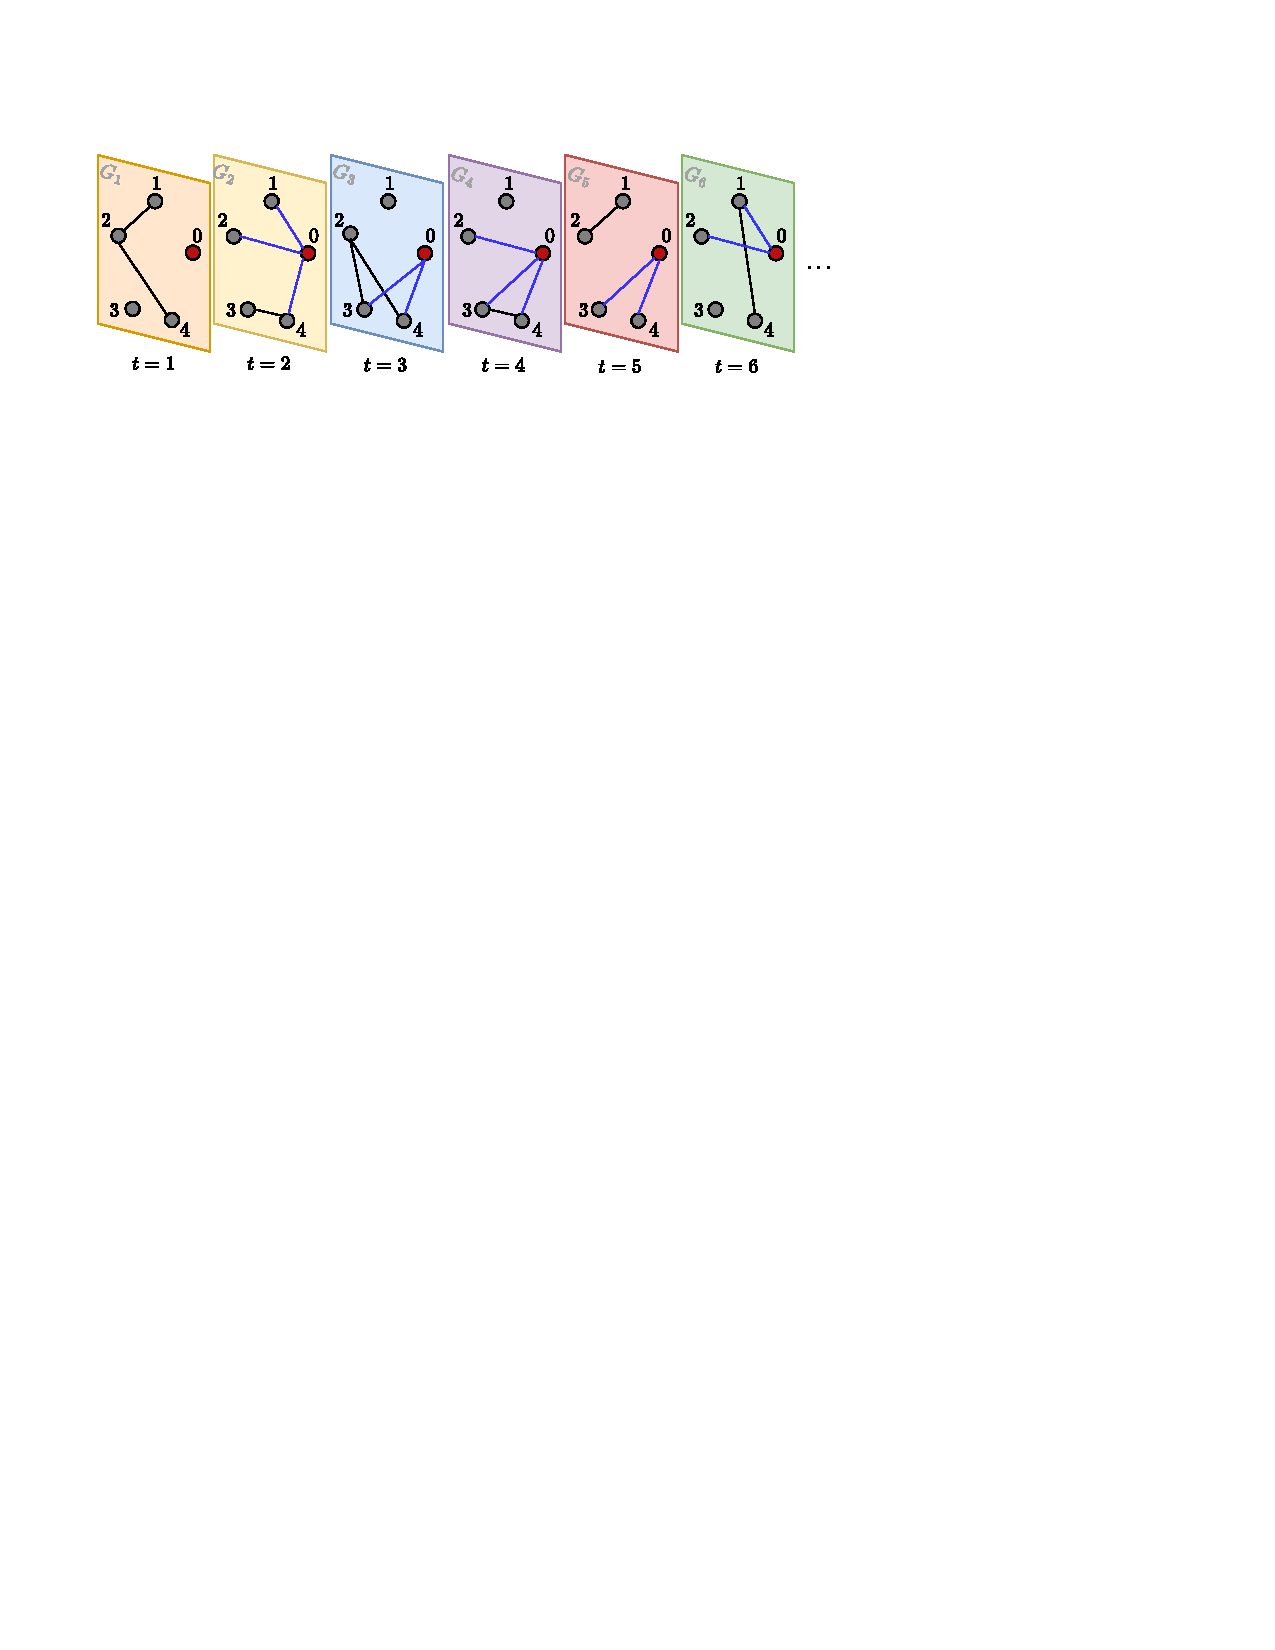
\includegraphics[width=\linewidth, height=8em, keepaspectratio]{figs/memory_node/lag=1.pdf}
    \caption{Illustration of a delayed cause-and-effect dataset with lag $\lag=1$. \underline{Black edges} show the cause subgraph (nodes 1 to $N$). \underline{\textcolor{blue}{Blue edges}} show the effect subgraph, where the memory node (0) connects to previously active cause nodes (degree $\geq$ 1). }
    \label{fig:memnode}
\end{figure}

\looseness-1 Intuitively, the model needs to remember nodes that were connected to each other at $E_{t-\ell}$ to predict the edges of the memory node at time $E_t$. An example of this task is illustrated in Figure~\ref{fig:memnode}. As \(\lag\) increases, the task becomes more challenging in terms of the memory capacity required from the model. While the number of nodes and edges in the graphs \(G_t\) also affect the task's difficulty, we focus on varying \(\lag\). Since only the edges involving the memory node can be predicted~(the other ones being completely random), only the $F_1$ over possible edges involving the memory node are reported in our experiments.

\looseness-1 \textbf{Task objectives and implementation.} In the delayed cause-and-effect tasks \(\causeeffect{\lag}\), TGNNs must propagate information across time steps while identifying the causal relationship governing the memory node's connectivity. This requires models to recognize temporal patterns and maintain historical information. The task difficulty scales with \(\lag\): larger values require retaining information longer, making causal relationship identification increasingly challenging. For implementation, we generate the underlying graphs (excluding the memory node) using an Erdős-Rényi model with 100 nodes and edge probability 0.01, creating a controlled environment to isolate and evaluate temporal reasoning capabilities.
\begin{figure}
    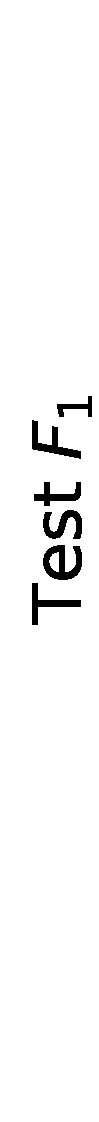
\includegraphics[width=0.04\linewidth]{kdd/figs/memory_node/(8, 6)/metric.pdf}
    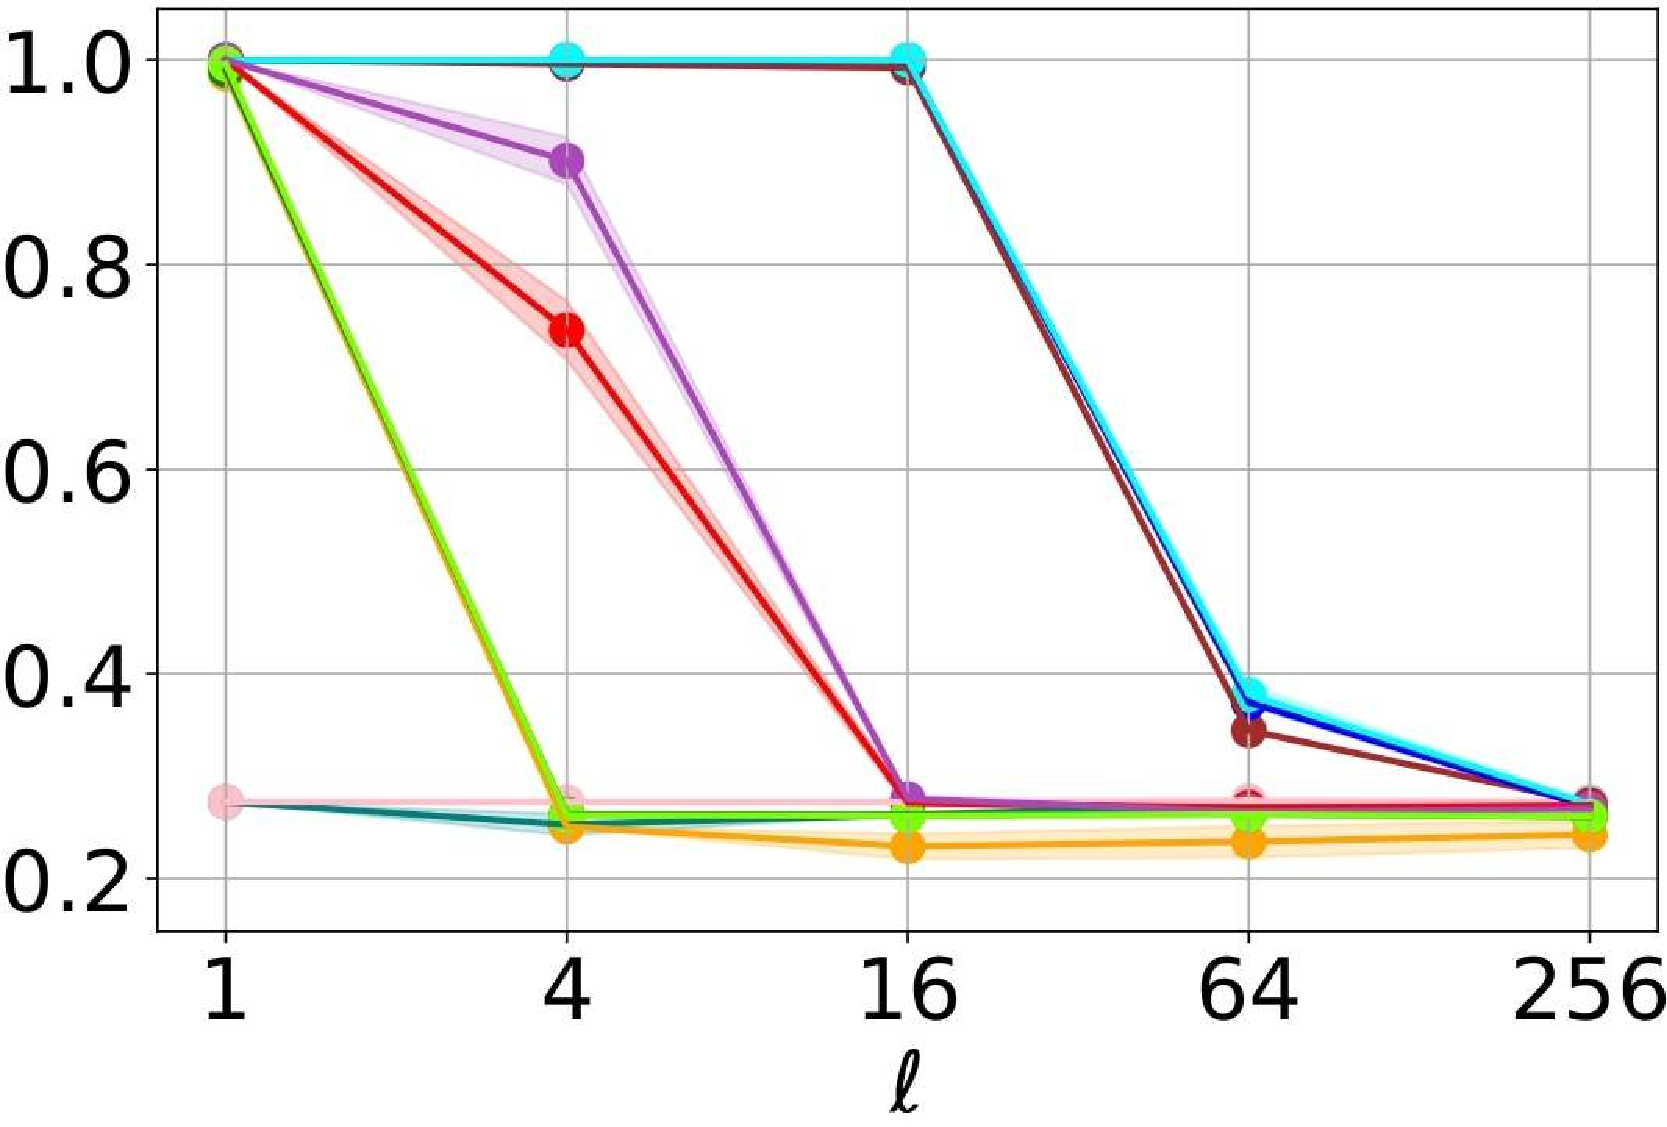
\includegraphics[width=0.6\linewidth]{figs/memory_node/(8, 6)/2(l).pdf}
    \hspace{0.5cm}\raisebox{5mm}{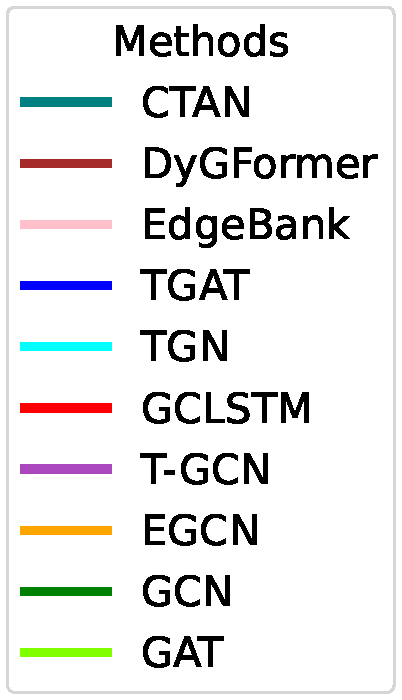
\includegraphics[width=0.2\linewidth]{figs/legends/CTDG DTDG all w edgebank wo persistence.pdf}}
        \caption{Methods' performance on cause-and-effect tasks $\causeeffect{\ell}$ across five temporal lags $\ell$.}
    \label{fig:plot_mem_node}
\end{figure}

\looseness-1 \textbf{Results.} Figure~\ref{fig:plot_mem_node} illustrates performance on cause-and-effect tasks across varying temporal lags. For minimal lags ($\ell = 1$), most methods demonstrate strong performance, as the task primarily requires extracting information from the immediate past, a capability even static models possess. However, as lag increases, performance degrades systematically, with static and DTDG approaches struggling significantly with longer temporal dependencies. GC-LSTM and T-GCN exhibit particularly pronounced performance deterioration at $\ell = 4$ and $\ell = 16$, revealing limitations in recurrent architectures' capacity to maintain long-term temporal information. Conversely, DyGFormer, TGAT, and TGN consistently outperform other methods, underscoring the efficacy of attention mechanisms and memory modules in capturing dynamic temporal patterns. At extended lags ($\ell = 64$ and $\ell = 256$), all methods converge toward EdgeBank's performance level, indicating a common challenge in modeling distant causal relationships. Notably, CTAN shows inconsistent performance even at minimal lags, suggesting inherent limitations in this context. These findings emphasize the crucial importance of architectural design choices, particularly attention and memory components, for effective temporal reasoning in dynamic graphs.
